% !TEX root = ../../thesis.tex

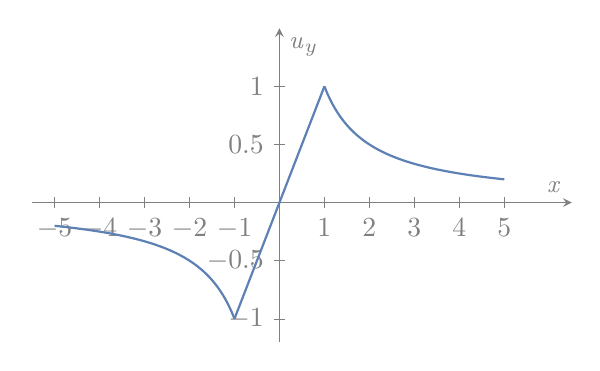
\begin{tikzpicture}
  \definecolor{mathematicaBlue}{rgb}{0.368417, 0.506779, 0.709798}
  \begin{axis}[
  axis x line=center, color=gray,
  axis y line=center, color=gray,
  xtick={-5,-4,...,5},
  ytick={-1,-0.5,...,1},
  xmin=-5.5,
  xmax=6.5,
  ymin=-1.2,
  ymax=1.5,
  x post scale=1,
  y post scale=0.7,
  xlabel=$\mbox{\small{\textit{x}}}$,
  ylabel=$\mbox{\small{\textit{u}}}_y$, 
  samples=200]
  \addplot[color=mathematicaBlue,thick,domain=1:5] {1/x};
  \addplot[color=mathematicaBlue,thick,domain=-5:-1] {1/x};
  \addplot[color=mathematicaBlue,thick,domain=-1:1] {x};
  \end{axis}
\end{tikzpicture}
